\chapter{Die ersten Schritte}
\epigraph{
	A little girl goes into a pet show and asks for a wabbit. The shop keeper looks down at her, smiles
	and says:\newline
	\enquote{Would you like a lovely fluffy little white rabbit, or a cutesy wootesly little brown rabbit?}\newline
	\enquote{Actually}, says the little girl, \enquote{I don't think my python would notice.}
}{Nick Leaton}

In diesem Abschnitt wollen wir unsere Arbeitsumgebung kennen lernen. Zu diesem Zweck werden wir ein sogenanntes \emph{Hello World} schreiben, \ie ein Programm, das lediglich den Text \texttt{Hello World!} auf dem Bildschirm ausgibt. Im Weiteren werden wir Python dazu benutzen, einfache Rechnungen umzusetzen.



\section{Der Kommandozeilen-Interpreter} \label{sec:Interpreter}
Wenn Sie eine \emph{Kommandozeilen-Umgebung} starten, können Sie Textkommandos an das Betriebssystem senden. Überwiegend handelt es sich dabei um die Anweisung, andere Programme auszuführen. Die Anweisung \texttt{python3}\footnote{Die Programmiersprache Python wurde seit ihrer Veröffentlichung im Jahre 1991 beständig weiterentwickelt. Manche Konzepte mussten komplett überarbeitet werden, so dass die einzelnen Versionen der Sprache nicht zwingend kompatibel miteinander sind. Wir arbeiten in der derzeit aktuellen Version 3.8. Auf einem Rechner können mehrere Python-Interpreter nebeneinander installiert sein. Daher müssen wir beim Aufruf die Versionsnummer 3 mit nennen.} ist ein solcher Befehl. Tippen Sie dies ein und drücken Sie \texttt{[ENTER]} um den Python-Interpreter zu starten.

Sie werden nun einen kurzen Versionstext sehen und hinter drei Pfeilen (\texttt{>{}>{}>}) einen blinkenden Cursor. Obwohl Sie noch immer dasselbe Fenster angezeigt bekommen, sind sie nun in der \emph{Interpreter-Umgebung}. Die Befehle, die Sie hier eingeben können, gehören zum Sprachumfang von Python!


\subsection{Hello World}
Ein solcher Befehl ist \inPy{print}. Er dient dazu, Informationen auf dem Bildschirm auszudrucken -- also genau das, was wir für unser Hello-World-Programm brauchen. Natürlich muss dazu auch angegeben werden, \emph{was} gedruckt werden soll. Wir müssen also einen Text \emph{als Argument übergeben}. Dies tun wir, indem wir den Text in Klammern () und Anführungszeichen \texttt{''''} einrahmen. Die Klammern dienen dazu, klar zu machen, was Argument ist, und was zum restlichen Code gehört. Die Anführungszeichen brauchen wir, um Text, der buchstäblich zu behandeln ist, von anderem Code abzutrennen. (Stellen Sie sich vor, sie wollten den Text \texttt{print} auf dem Bildschirm ausgeben. Der Computer versteht ohne Anführungszeichen den Unterschied zwischen dem Text \texttt{print} und dem Befehl \inPy{print} nicht. Vielleicht verstehen Sie nun den Anfang des Vorworts.) Geben Sie also ein:

\begin{center}
	\inPy{print("Hello World!")}
\end{center}

Der Interpreter reagiert prompt, und auf dem Bildschirm finden Sie exakt das, was Sie erwarten: Die Zeile \texttt{Hello World!}.

Nach den letzten Schritten sollten Sie also folgendes auf dem Bildschirm sehen:
\begin{cmdbox}[Starten des Python-Interpreters und Hello-World]
\begin{minted}{text}
blue-chameleon@blue-chameleon:~$ python3
Python 3.8.2 (default, Apr 27 2020, 15:53:34) 
[GCC 9.3.0] on linux
Type "help", "copyright", "credits" or "license" for more information.
>>> print("hello world!")
hello world!
\end{minted}
%$
\end{cmdbox}

Sollten Sie sich vertippen, wird ihnen dies in Form einer (anfangs etwas kryptischen) Fehlermeldung mitgeteilt:
\begin{cmdbox}[Eingabe mit Fehlern]
\begin{minted}{text}
>>> pirnt("hello world!")
Traceback (most recent call last):
  File "<stdin>", line 1, in <module>
NameError: name 'pirnt' is not defined
\end{minted}
\end{cmdbox}
Die letzte Zeile dieser Fehlermeldung teilt Ihnen mit, dass der Befehl \texttt{pirnt} nicht existiert. Sie werden diese Fehlermeldung sehr häufig bei Tippfehlern sehen, wie dies in diesem Beispiel der Fall war. Da Programme zum Teil sehr lang werden können, unterstützt Sie der Interpreter beim Debuggen, indem in der vorletzten Zeile der Ausgabe die Stelle genannt wird, an der die fehlerhafte Eingabe stattfand: \texttt{line 1} sagt, dass die erste Zeile dieses Codes fehlerhaft war.

Vergessen wir beispielsweise, die Anführungszeichen abzuschließen, erhalten wir eine ähnliche Fehlermeldung:

\begin{cmdbox}[Eingabe mit Fehlern]
\begin{minted}{text}
>>> print("hello world)
  File "<stdin>", line 1
    print("hello world)
                      ^
SyntaxError: EOL while scanning string literal
\end{minted}
\end{cmdbox}
\texttt{EOL} steht für \emph{end of line}: Bevor der \emph{string literal} (also unser Text) durch ein abschließendes Anführungszeichen beendet wurde, endete die Zeile.

Ein interessantes Verhalten erzielen Sie, wenn Sie die abschließende Klammer vergessen: Argumente in Python dürfen sich über mehrere Zeilen erstrecken. Anstatt eine Fehlermeldung zu zeigen, wird der Interpreter Sie über drei Punkte (\texttt{...}) auffordern, die Zeile fortzusetzen. Wenn Sie hier die Klammer nachträglich schließen, erhalten Sie die erwartete Ausgabe:
\begin{cmdbox}[Eingabe über mehrere Zeilen]
\begin{minted}{text}
>>> print("hello world"
... )
hello world
\end{minted}
\end{cmdbox}

Mit dem Befehl
\begin{center}
	\inPy{quit()}
\end{center}
beenden Sie den Kommandozeilen-Interpreter wieder; sie sind nun wieder in der Umgebung Ihres Betriebssystems, wo Sie also \emph{keine} Python-Befehle mehr eingeben können.



\section{Script-Dateien} \label{sec:Scripts}
Mit dem letzten Abschnitt haben Sie den ersten Python-Befehl \inPy{print} kennen gelernt! In den Kommandozeilen-Interpreter eingegeben bewirkt er eine direkte Ausgabe auf dem Bildschirm. Sie werden sehr bald weitaus komplexere Programme schreiben, für die es umständlich wäre, sie Zeile für Zeile für jede Ausführung neu einzugeben.

Stattdessen können Sie ein \emph{Textdokument} anlegen, in dem Sie alle Anweisungen nacheinander eingeben und speichern, und den Interpreter anschließend dazu auffordern, diese Datei zu lesen und den Code darin auszuführen. Wichtig hierbei ist, dass es sich wirklich um eine \emph{reine Textdatei} handelt, dass also keine Formatierungen oder sonstigen Inhalte enthält, die über den reinen Code hinaus gehen. Verwenden Sie also zum Schreiben von Code \emph{nicht} Programme wie Word, LibreOffice o.\,ä., sondern Code/Text-Editoren. Ich empfehle:
\begin{itemize}
\item für Linux
	\begin{itemize}
	\item kate (KDE-Editor): auf die Arbeit mit vielen Programmiersprachen ausgelegt, sehr lightweight
	\item gedit: oft vorinstalliert, minimale Features aber alles notwendige gegeben
	\item geany: auf größere Projekte ausgelegt, aber immer noch hinreichend Ressourcen schonend
	\end{itemize}
\item für Windows
	\begin{itemize}
	\item Notepad++: Bietet alle Funktionalitäten, die das Programmieren angenehm machen, 
		ohne dabei zu viele Systemressourcen zu verbrauchen.\\
		Siehe \url{https://notepad-plus-plus.org/}
	\item Notepad: Immer vorinstalliert. Die Arbeit mit diesem Programm ist oft mühselig, da Features
		wie Syntax Highlighting oder Automatische Einrückung nicht gegeben sind; dafür muss nichts
		installiert werden
	\end{itemize}
\end{itemize}

In diesen (und etwa einer Million weiteren) Editoren können Sie Code verfassen und als \texttt{*.py}-Datei abspeichern. Aus der Kommandozeile können Sie diesen Code an den Interpreter weitergeben, indem Sie eingeben:
\begin{center}
\texttt{python3 [myCode].py}
\end{center}
Wobei \texttt{[myCode]} selbstverständlich durch den von Ihnen vergebenen Dateinamen ersetzt werden muss.


\subsection{Beispiel}
Schreiben Sie den folgenden Code in eine Textdatei, und speichern Sie diese als \texttt{HelloWorld.py} ab. (Achten Sie auch auf Groß/Kleinschreibung).
\begin{codebox}[Datei \texttt{HelloWorld.py}]
\begin{minted}[linenos]{python}
print("Hello World!")
\end{minted}
\end{codebox}

Starten Sie eine Kommandozeilen-Umgebung, und wechseln in dieser in das Verzeichnis, unter dem Sie die Datei abgespeichert haben\footnote{Stichwort \texttt{cd}. Falls Sie nicht wissen, wie das geht, sprechen Sie bitte Ihre Dozenten an.}. In diesem Fall sei der Code unter \texttt{\textasciitilde/Codes} abgelegt. Zum Ausführen dieses Codes geben Sie also ein:

\begin{cmdbox}[Starten des Python-Interpreters und Hello-World]
\begin{minted}{text}
blue-chameleon@blue-chameleon:~$ cd Codes/
blue-chameleon@blue-chameleon:~/Codes$ python3 HelloWorld.py 
Hello World!
\end{minted}
\end{cmdbox}



\section{IDEs}
Neben der Arbeit mit Texteditoren, die vom Interpreter abgegrenzt stehen, existieren auch IDEs, also \emph{Integrated Development Environments}. Es handelt sich dabei um Programme, die eine direkte Anbindung an den Interpreter haben und somit Code-Schreiben und Ausführen im selben Fenster erlauben.

Viele empfinden es als bequemer, mit IDEs zu arbeiten. Diese Programme sind oft aber auch etwas aufwändiger gebaut, und brauchen länger, bis sie geladen sind. Experimentieren Sie hier selbst, welcher Modus Ihnen am besten zusagt; für den Kurs sind beide Wege -- Text-Editor und IDE -- gangbare Wege.

Ich empfehle die IDE spyder3. Linux-User können diese einfach aus dem Paketverwaltungssystem heraus installieren; Windows-User mögen von \url{https://www.spyder-ide.org/} die Installationspakete herunterladen.

\begin{figure}
	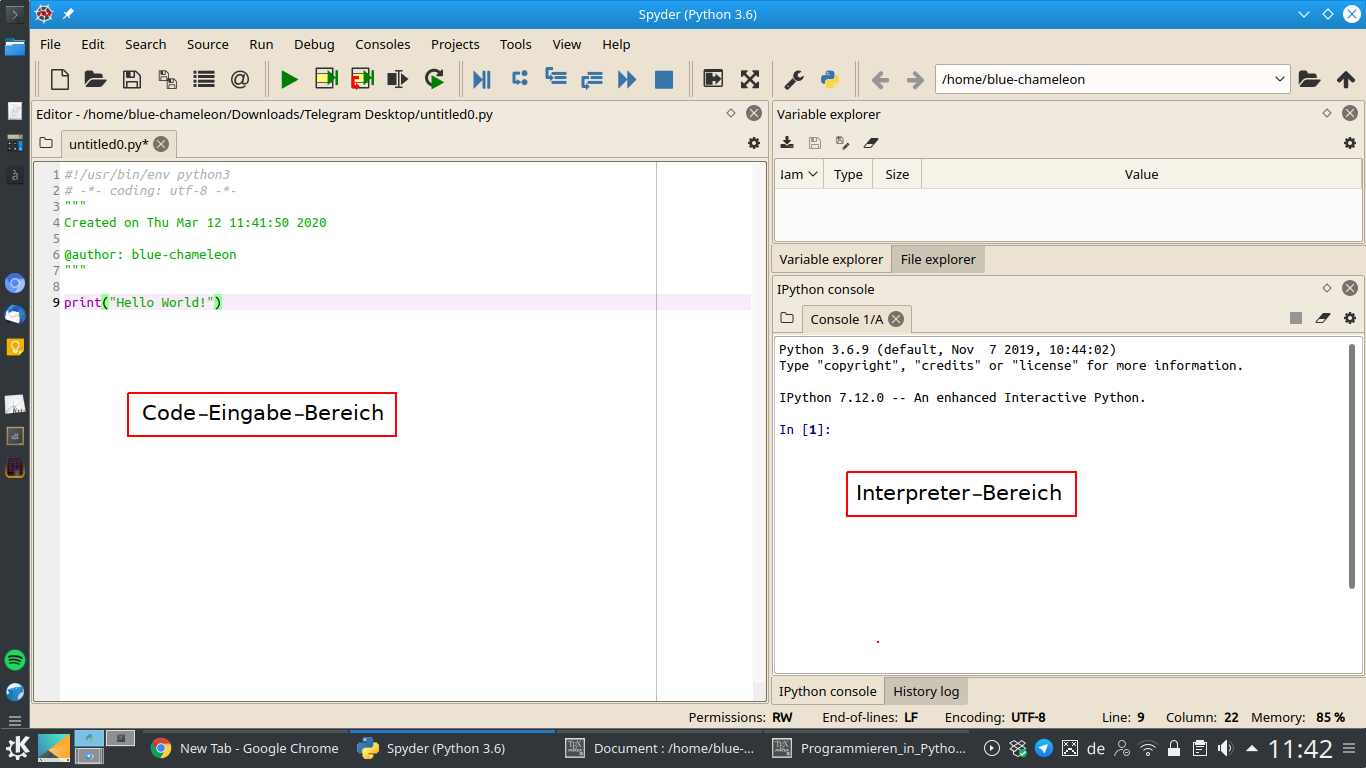
\includegraphics[width=\linewidth]{./gfx/Spyder}
	\caption{Die IDE Spyder} \label{gfx:Spyder}
\end{figure}

In Abbildung \ref{gfx:Spyder} sehen Sie die Arbeitsumgebung des Programms Spyder. Insbesondere finden Sie links einen größeren Bereich, in dem sie komplexere Codes schreiben können, wie schon in Abschnitt \ref{sec:Scripts} angedeutet. In der rechten Fensterhälfte sehen Sie den Interpreter-Bereich, in den Sie direkt Python-Kommandos eingeben können. Genauso, wie in Abschnitt \ref{sec:Interpreter} gezeigt, werden die Befehle, die Sie hier eintippen, sofort ausgeführt.



\section{Rechnen}
Wie erwähnt können wir Python dazu benutzen, einfache Berechnungen ausführen zu lassen. Dazu tippen wir diese einfach direkt in die Interpreter-Umgebung ein:
\begin{cmdbox}[Python als \enquote{Taschenrechner}]
\begin{minted}{text}
>>> 1 + 2
3
\end{minted}
\end{cmdbox}

Diese Rechnungen dürfen aus beliebig vielen Operationen bestehen, halten sich an die Regel \enquote{Punkt vor Strich} und können auch Klammern enthalten:
\begin{cmdbox}[Python als \enquote{Taschenrechner}]
\begin{minted}{text}
>>> ((1 - 5) * 3) / (4 + 1) ** 2
-0.48
\end{minted}
\end{cmdbox}

Dabei werden folgende Zeichen als Operatoren verstanden:
\begin{table}[h!]
\newcolumntype{O}{>{\centering\ttfamily\arraybackslash}m{.2 \textwidth}}
\newcolumntype{F}{>{\centering         \arraybackslash}m{.6 \textwidth}}
\newcolumntype{X}{>{\centering\ttfamily\arraybackslash}m{.2 \textwidth}}

\rowcolors{1}{white}{tabhighlight}
\begin{tabularx}
	{\linewidth}
	{OFX}
	\toprule[1.5pt]

	\normalfont	\bfseries Zeichen &
				\bfseries Funktion &
				\bfseries Beispiel
	\tabcrlf
	+  & Addition					& 1 + 2 = 3 \tabcrlf
	-  & Subtraktion					& 5 - 7 = -2 \tabcrlf
	*  & Multiplikation				& 2 * 4 = 8 \tabcrlf
	/  & Division					& 7 / 5 = 1.4 \tabcrlf
	// & Ganzzahl-Division			& 7 // 5 = 1 \tabcrlf
	\% & Modulo (Rest der Division)	& 7 \% 5 = 2 \tabcrlf
	** & Potenzierung				& 3 ** 2 = 9 \\
	
	\bottomrule[1.5pt]	
\end{tabularx}
\caption{Rechenoperatoren in Python}
\end{table}

Auch das Rechnen mit \emph{komplexen Zahlen} ist möglich. Als imaginäre Einheit wird das Zeichen \inPy{j} verwendet:
\begin{cmdbox}[Komplexe Zahlen]
\begin{minted}{text}
>>> (1j)**2
(-1+0j)
\end{minted}
\end{cmdbox}
Wie Sie sehen, wird das Ergebnis von Rechnungen mit komplexen Zahlen als komplexe Zahl ausgegeben, selbst wenn die Zahl rein reell ist. Mehr dazu im Abschnitt \ref{sub:datatypes}.


\subsection{Variablen}
Die Ergebnisse einer Rechnung können in \emph{Variablen} gespeichert werden. Es handelt sich hierbei um Speicherstellen, denen Sie einen mehr oder minder beliebigen Namen geben können:
\begin{cmdbox}[Variable für Zwischenergebnisse]
\begin{minted}{text}
>>> x = 3 + 7
>>> x ** 2
100
\end{minted}
\end{cmdbox}

Variablen können einzelne Buchstaben sein, dürfen aber auch ganze Worte zum Namen haben. Im Variablennamen dürfen auch der Unterstrich (\_) und die Ziffern 0-9 vorkommen; jedoch muss das erste Zeichen ein Buchstabe sein. Python ist \emph{case sensitive}, \ie zwischen Groß- und Kleinschreibung wird unterschieden.

\begin{table}[h!]
\newcolumntype{O}{>{\centering\ttfamily\arraybackslash}m{.3 \textwidth}}
\newcolumntype{F}{>{\centering         \arraybackslash}m{.3 \textwidth}}
\newcolumntype{X}{>{\centering         \arraybackslash}m{.5 \textwidth}}

\rowcolors{1}{white}{tabhighlight}
\begin{tabularx}
	{\linewidth}
	{OFX}
	\toprule[1.5pt]

	\normalfont	\bfseries Name &
				\bfseries Erlaubt &
				\bfseries Begründung
	\tabcrlf
	x  						& ja 	& \tabcrlf
	counter					& ja 	& \tabcrlf
	CounTer					& ja 	& \tabcrlf
	number\_of\_elements		& ja 	& \tabcrlf
	list4					& ja 	& \tabcrlf
	5th\_list 				& nein	& Ziffer als erstes Zeichen \tabcrlf
	list 4 					& nein	& Leerzeichen \tabcrlf
	Best\_List\_Ever!		& nein	& Rufezeichen \tabcrlf
	print					& Problematisch	& überschreibt den Befehl print\\
	
	\bottomrule[1.5pt]	
\end{tabularx}
\caption{Beispiele für Variablen in Python}
\end{table}

\begin{hintbox}[Sprechende Variablennamen]
Ihre Programme werden sehr bald einige Komplexität annehmen. Sie sollten daher Variablen so benennen, dass auf den ersten Blick erkennbar wird, welche Art Information gespeichert wird. Der Name \inPy{ListLength} ist in jedem Fall dem Namen \inPy{l} vorzuziehen.
\end{hintbox}
%
\begin{hintbox}[Schlüsselworte]
Die Liste oben nennt das Symbol \inPy{print} als erlaubten, aber problematischen Namen. Tatsächlich können Sie in Python die Sprachelemente umdefinieren, und so etwa \inPy{print} als Variable benutzen oder eine andere Routine unter diesem Namen aufrufen. Im Sinne von Lesbarkeit und Kompatiblität mit anderen Programmen sollten Sie hiervon aber Abstand nehmen! Wenn Sie \inPy{print} überschreiben, können Sie zunächst nichts mehr auf dem Bildschirm ausgeben.

Da Sie gerade erst beginnen, die Sprache Python zu erlernen, können Sie natürlich noch nicht alle Symbole kennen, die bereits vergeben sind. Wenn Sie einen Editor mit Syntax-Highlighting verwenden, können Sie aber \idR diese farblichen Markierungen zur Hilfe nehmen: Wenn der Editor ihr Symbol wie einen Befehl markiert, sollten Sie es umbenennen. Wird keine besondere Farbe zugewiesen, so ist der Name vermutlich noch frei. Einige Schlüsselworte sind besonders geschützt, und können nicht überschrieben werden. Sie erhalten die Fehlermeldung \texttt{SyntaxError: invalid syntax}, falls Sie versuchen, ein solches Schlüsselwort als Variablenname zu verwenden.
\end{hintbox}

\begin{hintbox}[Unterstriche in Variablennamen]
Variablennamen dürfen prinzipiell an jeder Stelle Unterstriche enthalten, auch als erstes Zeichen. Es ist aber Konvention, dies nur in bestimmten Situationen zu tun, auf die ich an gegebener Stelle erst eingehen werde. Vermeiden Sie daher vorerst Namen wie \inPy{_var}.
\end{hintbox}

\begin{hintbox}[Non-ASCII-Variablennamen (Umlaute{,} Sonderzeichen{,} \ldots)]
Python 3 erlaubt es prinzipiell, Variablennamen aus dem UTF-8-Zeichenvorrat zu wählen. Das bedeutet, dass neben den lateinischen Klein- und Großbuchstaben (a-z, A-Z) auch Umlaute, Zeichen mit Akzenten, griechische, japanische, \ldots Zeichen für Variablennamen erlaubt sind. Dies führt aber schnell zu Kompatibilitätsproblemen. Neben den offensichtlichen Problemen -- Kollegen in anderen Ländern könnten die Schriftzeichen, die zur Bedienung Ihres Codes nötig sind, nicht eingeben können -- ist manchmal schon das Versenden und Ausführen von Code auf einem anderen Rechner in derselben Arbeitsgruppe schwierig.

Während Python also Variablennamen wie \inPy{äußerstWichtig} durchaus erlaubt, sollten Sie also dennoch nur auf den englischen Zeichenvorrat zurückgreifen, und eine Variable beispielsweise \inPy{exceptionallyImportant} benennen.
\end{hintbox}

Variablen können aktualisiert (\ie überschrieben werden). Dies kann auch mit Bezug auf den alten Wert derselben Variable geschehen:
\begin{cmdbox}[Variable für Zwischenergebnisse]
\begin{minted}{text}
>>> x = 1
>>> x
1
>>> x = 2
>>> x
2
>>> x = x + 1
>>> x
3
\end{minted}
\end{cmdbox}

\begin{warnbox}[Python ist kein Gleichungslöser]
Für mathematisch denkende KursteilnehmerInnen mag die Zeile \inPy{x = x + 1} unsinnig wirken. Offensichtlich gibt es keine Zahl \inPy{x}, die diese Gleichung erfüllt. In Python beschreiben wir auf diese Art aber auch keine Gleichung, sondern einen Arbeitsauftrag: Speichere in der Variable \inPy{x} den Wert der Summe des aktuellen Werts von \inPy{x} plus 1!

Denken Sie an das Vorwort bei der Arbeit mit Computern: Maschinen verstehen komplexe Aufgaben wie das Lösen eines Gleichungssystems nicht.
\end{warnbox}

\begin{hintbox}[Shorthands]
Das Aktualisieren eines Werts unter Bezug auf den alten Wert ist ein häufiger Arbeitsschritt beim Programmieren. Daher wurden Abkürzungen (Shorthands) eingeführt. So steht zum Beispiel der Ausdruck
\begin{center}
	\inPy{x += 1}
\end{center}
für den Code
\begin{center}
	\inPy{x = x + 1}
\end{center}
Ähnlich sind auch \inPy{x -= y}, \inPy{x *= y}, usw. erlaubt.
\end{hintbox}

Die Werte von Variablen können in einem Schritt getauscht werden, indem wir ein Komma zur Hilfe nehmen:
\begin{cmdbox}[Variable für Zwischenergebnisse]
\begin{minted}{text}
>>> x = 1
>>> y = 2
>>> x, y = y, x
>>> x
2
>>> y
1
\end{minted}
\end{cmdbox}
Ein \emph{Dreieckstausch} (\ie die Zuhilfe-Nahme einer dritten Variable) ist nicht nötig. (Intern führt Python einen Dreieckstausch aus; dies wird aber automatisch für Sie erledigt, ohne weiteres zutun Ihrerseits).


\subsection{Datentypen} \label{sub:datatypes}
In diesem Abschnitt arbeiten wir mit Zahlen. Für Sie als Mensch ist eine Zahl eindeutig durch ihren Wert bestimmt: 1 = 1.0 = 1 + 0j = eins. Ein Computer \enquote{kennt} aber zunächst keine Werte, sondern nur binäre Information. Einer Folge von Einsen und Nullen kann nicht angesehen werden, ob diese jetzt eine ganze Zahl, eine komplexe Zahl, einen Teil eines Bildes oder eine Anweisung eines Computerprogramms darstellen. Daher wird jeder Information ein \emph{Datentyp} zugeordnet, also eine Anweisung, wie die Folge von Einsen und Nullen zu interpretieren ist.

Vorerst beschäftigen wir uns mit vier Datentypen:
\begin{itemize}
\item \inPy{int} -- Ganzzahlen, also \inPy{0}, \inPy{1}, \inPy{2}, \inPy{3}, 
		\ldots, sowie negative Ganzzahlen
\item \inPy{float} -- Fließkommazahlen, also \inPy{3.14} oder \inPy{1.0}. (Beachten Sie: als
		Dezimaltrennzeichen verwenden wir einen \emph{Punkt}, kein Komma.)
\item \inPy{complex} -- Komplexe Zahlen, also \inPy{(1+2.7j)}
\item \inPy{str} -- Strings, also Zeichenketten wie \inPy{"Hallo Welt"}
\end{itemize}

Der Datentyp eines Werts wird bei seiner \enquote{Berechnung} festgelegt und zusammen mit der Variablen gespeichert, über die der Wert Verfügbar gehalten wird. Dabei gilt die Grundregel, dass keine Information verloren gehen darf. Bei der Addition einer Ganzzahl (\inPy{int}) und einer Fließkommazahl (\inPy{float}) darf beispielsweise die Information über die Nachkomma-Anteil nicht verloren gehen (selbst, wenn dieser \inPy{.0} ist). Betrachten Sie hierzu folgendes Beispiel:

\begin{cmdbox}[Datentypen bei Addition]
\begin{minted}{text}
>>> 1 + 1
2
>>> 1.0 + 1
2.0
>>> 1 + 1.0
2.0
>>> 1.0 + 1.0
2.0
\end{minted}
\end{cmdbox}

In der ersten Zeile (\inPy{1 + 1}) sind nur Ganzzahlen beteiligt. Somit ist das Ergebnis auch eine Ganzzahl, und wird folgerichtig als solche (\ie ohne Nachkommastelle) ausgegeben. In allen anderen Fällen ist immer mindestens eine Fließkommazahl beteiligt; das Ergebnis ist daher immer \inPy{2.0} (nicht nur \inPy{2}).

Bei der Division wird immer eine Fließkommazahl berechnet, egal ob die Argumente vom Typ \inPy{int} oder \inPy{float} sind.

Ähnlich verhält es sich bei komplexen Zahlen: Sobald eine komplexe Zahl an der Rechnung beteiligt ist, wird auch das Ergebnis vom Typ \inPy{complex} sein. Da \inPy{complex}-Werte auch Nachkomma-Werte speichern können, übertrifft diese Regel die bzgl. \inPy{float}s.

Wenn Sie sich nicht sicher sind, welchen Datentyp eine Variable hat, können Sie den Befehl
\begin{center}
	\inPy{type(Ausdruck)}
\end{center}
benutzen. Dabei steht \inPy{Ausdruck} für eine Variable, eine Zahl oder eine komplette Rechnung.

\begin{cmdbox}[Beispiele zu \texttt{type} (1)]
\begin{minted}{text}
>>> type(1)
<class 'int'>
>>> type(1.0)
<class 'float'>
>>> type(1j)
<class 'complex'>
>>> type(1+1.0)
<class 'float'>
>>> a=1j**2
>>> type(a)
<class 'complex'>
>>> a
(-1+0j)
\end{minted}
\end{cmdbox}

Wollen Sie erzwingen, dass das Ergebnis in einen bestimmten Typ umgewandelt wird, so können Sie den Datentyp vor einen Ausdruck setzen, und diesen einklammern:
\begin{center}
	\inPy{Datentyp(Ausdruck)}
\end{center}

Dabei können Informationen verloren gehen:
\begin{cmdbox}[Beispiele zu \texttt{type} (2)]
\begin{minted}{text}
>>> a = int(1 + 1.9)
>>> type(a)
<class 'int'>
>>> a
2
\end{minted}
\end{cmdbox}
in diesem Beispiel etwa wird der Nachkommaanteil abgeschnitten.

Wie bereits erwähnt, sind Strings (Zeichenketten) dadurch erkennbar, dass ihr Inhalt durch doppelte Anführungszeichen (''\ldots'') vom restlichen Code abgegrenzt wird. Alternativ können auch einfache Anführungszeichen ('\ldots') verwendet werden. Dies hat den Zweck, es Programmierern einfach zu machen, Strings zu Erzeugen, in denen auch selbst wieder Anführungszeichen vorkommen.

\begin{cmdbox}[Beispiele zu Strings (1)]
\begin{minted}{text}
>>> 'abc'
'abc'
>>> "abc"
'abc'
>>> "abc'def'ghi"
"abc'def'ghi"
>>> 'abc"def'
'abc"def'
\end{minted}
\end{cmdbox}

Auch mit Strings kann \enquote{gerechnet} werden; hier sind jedoch nur die Addition (\inPy{+}) und die Multiplikation (\inPy{*}) mit Ganzzahlen definiert. Die Addition verkettet zwei Strings; die Multiplikation wiederholt einen String mehrere Male:

\begin{cmdbox}[Beispiele zu Strings (2)]
\begin{minted}{text}
>>> "ab" + 'cd'
'abcd'
>>> 3 * "ab"
'ababab'
>>> 0 * "ab"
''
>>> "ab" + "'c'def"
"ab'c'def"
\end{minted}
\end{cmdbox}

Die Befehle \inPy{int}, \inPy{float}, \inPy{complex} können -- in begrenztem Maße -- auch auf Strings angewandt werden:

\begin{cmdbox}[Konversion von Strings zu Zahlentypen]
\begin{minted}{text}
>>> int("1")
1
>>> int("1.3")
Traceback (most recent call last):
  File "<stdin>", line 1, in <module>
ValueError: invalid literal for int() with base 10: '1.3'
>>> float("1.3")
1.3
>>> float("1,3")
Traceback (most recent call last):
  File "<stdin>", line 1, in <module>
ValueError: could not convert string to float: '1,3'
>>> complex("1j")
1j
>>> int("one")
Traceback (most recent call last):
  File "<stdin>", line 1, in <module>
ValueError: invalid literal for int() with base 10: 'one'
\end{minted}
\end{cmdbox}

Wie Sie sehen, wird die Darstellung als Text in Zahlen zurückverwandelt, sofern das für den gewünschten Zieltyp möglich ist; andernfalls erhalten Sie eine Fehlermeldung.

Machen Sie sich klar: Für den Computer sind Text und Zahlen unterschiedliche Informationen! Eine \emph{semantische} Interpretation ist nicht möglich. Machen Sie sich daher auch klar, was der Unterschied zwischen diesen drei Additionen ist:
\begin{cmdbox}[Strings und \texttt{int}s (1)]
\begin{minted}{text}
>>> x = "1"
>>> y = "2"
>>> x + y
'12'
>>> int(x + y)
12
>>> int(x) + int(y)
3
\end{minted}
\end{cmdbox}

Wir beginnen mit den \emph{String}-Variablen \inPy{x} und \inPy{y}. Die Addition von Strings ist gleichbedeutend mit der Verkettung; daher ist das Ergebnis von \inPy{x + y} auch folgerichtig der \emph{String} \inPy{"12"}.

Der Aufruf von \inPy{int} in \inPy{int(x + y)} erhält als Argument den Wert \texttt{x + y}, also den \emph{String} \inPy{"12"}. Folgerichtig wird die \emph{Zahl} \inPy{12} berechnet.

Im dritten Teilbeispiel \inPy{int(x) + int(y)} dagegen werden separat die Zahlen \inPy{1} und \inPy{2} aus den Variablen \inPy{x} und \inPy{y} berechnet, und diese dann addiert. Entsprechend kann erst hier das Ergebnis die Zahl \inPy{3} sein.

Natürlich können Sie auch beliebige Zahlen in Strings umwandeln; dazu verwenden Sie einfach den Befehl \inPy{str}:

\begin{cmdbox}[Strings und \texttt{int}s (2)]
\begin{minted}{text}
>>> x = 1
>>> y = 2
>>> str(x + y)
'3'
>>> str(x) + str(y)
'12'
\end{minted}
\end{cmdbox}

\begin{hintbox}[Sprechweise: \emph{dynamische Typisierung} und \emph{duck-typing}]
In vielen Programmiersprachen wird der Datentyp von Variablen einmal festgelegt und darf sich dann für das weitere Programm nicht mehr ändern. Python dagegen erlaubt \emph{dynamische Typisierung}: Eine Variable \inPy{x} kann an einer Stelle des Programms Ganzzahlen speichern und an späterer Stelle Strings. Damit einher geht eine gewisse Ambivalenz; es ist nicht zwingend sofort einsichtig, welchen Datentyp ein Ausdruck hat. Der Python-Interpreter versucht dann, den geeignetsten Datentyp zu \enquote{erraten}. Gemäß dem Zitat von James Whitcomb Riley:
\begin{tcolorbox}[title=Zitat]
When I see a bird that walks like a duck and swims like a duck and quacks like a duck, I call that
bird a duck.
\end{tcolorbox}
wird Python daher als \emph{duck typed language} bezeichnet.
\end{hintbox}


\subsection{Ausgabe von Variablen mit \inPy{print}}
Um den in einer Variablen gespeicherten Wert zu erfahren, haben wir bisher in der Interpreter-Umgebung den Namen der Variable eingegeben. In längeren Codes, wie wir sie im Code-Eingabe-Bereich schreiben, funktioniert dies aus technischen Gründen leider nicht. Stattdessen können wir aber den \inPy{print} benutzen. Betrachten Sie das folgende Beispiel:

\begin{codebox}[Beispiel: Ausgabe von Werten mit \texttt{print}]
\begin{minted}[linenos]{python}
a = 2
b = a * 7.5 + 2
print(a, b, "konstanter Text", a * "x")
\end{minted}
\end{codebox}

\begin{cmdbox}[Ausgabe: Ausgabe von Werten mit \texttt{print}]
2 17.0 konstanter Text xx
\end{cmdbox}

Sie erkennen hieraus, dass Sie der Befehl \inPy{print} die \emph{Werte der Ausdrücke, die als Argumente übergeben werden}, ausgibt. Das bedeutet, dass \inPy{a} eben durch seinen Wert (hier also durch \inPy{2}) ersetzt wird. Ich erinnere Sie nochmals daran, dass dies der Grund ist, warum Strings in Anführungszeichen eingefasst werden müssen -- sonst könnte der Interpreter die Anweisung \emph{drucke den Buchstaben a} und die Anweisung \emph{drucke den Wert der Variablen }\inPy{a} nicht auseinander halten.

Weiter sehen Sie, dass \inPy{print} nicht nur einen einziges Argument verarbeiten kann, sondern auch mit einer ganzen \emph{Parameterliste} zurecht kommt. Die einzelnen Ausdrücke werden durch Kommata gelistet aufgelistet und der Reihe nach ausgewertet, bevor sie auf dem Bildschirm erscheinen. Diese Ausdrücke dürfen einzelne Variablen (\inPy{a}, \inPy{b}), Konstanten (\inPy{3.14}, \inPy{"konstanter Text"}) oder komplette \enquote{Rechnungen} (\inPy{a * "x"}) sein.



\section{Kommentare und mehrzeilige Kommandos}
Wie Sie bald sehen werden, können Codes lang und komplex werden. Es wird Ihnen helfen, schwer erfassbare Abschnitte durch Fließtext-Kommentare zu ergänzen. Solche Kommentare markieren Sie durch ein Raute-Zeichen (\#). Der Interpreter wird alle Zeichen hinter dem Kommentar-Zeichen bis zum Zeilenende ignorieren.

\begin{codebox}[Beispiel: Kommentare]
\begin{minted}[linenos]{python}
print("Normaler Code, der ausgeführt wird")  # Dies wird nicht mehr ausgeführt
#print("auch dies wird nicht ausgeführt")
\end{minted}
\end{codebox}

Normalerweise enden Python-Anweisungen mit dem Zeilenumbruch. An manchen Stellen kann es Ihren Code übersichtlicher machen, Anweisungen auf mehrere Zeilen zu verteilen. Dass eine Anweisung trotz Zeilenumbruch über das Zeilenende gelesen werden soll, erreichen Sie, indem Sie einen Backslash (\textbackslash) setzen:

\begin{codebox}[Beispiel: Mehrzeilige Anweisungen]
\begin{minted}[linenos]{python}
x = 1
a = 2 + \
    3 * x + \
    4 * x**2 + \
    7 * x**3
\end{minted}
\end{codebox}


\section{Formatierte Strings}
Wir können Strings erzeugen, in denen die Werte von Variablen als Text dargestellt werden. Zu diesem Zweck haben wir bereits die Funktion \inPy{str} kennengelernt. Wir wissen auch, dass wir Strings durch die Addition verketten können. Ein bequemerer Weg kann über \emph{Format-Strings} erreicht werden:
\begin{codebox}[Syntax: Format-String]
\begin{minted}{python}
f"normaler Text {Ausdruck} mehr normaler Text {weiterer Ausdruck:Format} ..."
\end{minted}
\end{codebox}

Ein Format-String beginnt also mit einem vorangestellten \inPy{f}, und wird ebenso von doppelten Anführungszeichen \inPy{""} eingeschlossen, wie ein normaler String. Er kann -- muss aber nicht -- beliebig lange Blocks von Text enthalten, die 1:1 in das Endergebnis übernommen werden. Neu gegenüber normalen Strings sind Blöcke der Form \inPy{{Ausdruck}} und \inPy{{Ausdruck : Format}}.

Wie schon zuvor auch steht \inPy{Ausdruck} für eine Variable, eine Zahl oder eine komplette Rechnung. Der Ausdruck wird zuerst \emph{evaluiert} (\enquote{ausgerechnet}), und dann in den String eingebaut. Die \{geschweiften Klammern\} sind nicht Teil des Endprodukts, sondern zeigen dem Interpreter an, dass hier eine Ersetzung gemacht werden muss.

\begin{codebox}[Beispiel: Formatstrings]
\begin{minted}[linenos]{python}
a = 1
b = 2
s = f"a + b = {a + b}"
print(s)
\end{minted}
\end{codebox}

\begin{cmdbox}[Ausgabe: Formatstrings]
a + b = 3
\end{cmdbox}

Dieser Code ist im Ergebnis gleichwertig zu 
\begin{codebox}[Beispiel: Gleichwertiger Code ohne Formatstrings]
\begin{minted}[linenos]{python}
a = 1
b = 2
s = "a + b = " + str(a + b)
print(s)
\end{minted}
\end{codebox}

Wenn Sie tatsächlich \{geschweifte Klammern\} im Ergebnis brauchen, so erreichen sie dies, indem Sie im Formatstring ein doppeltes Klammerpaar setzen:
\begin{codebox}[Beispiel: Formatstrings mit Escape-Sequenz]
\begin{minted}[linenos]{python}
a = 1
b = 2
s = f"{{a + b}} = {{{a + b}}}"
print(s)
\end{minted}
\end{codebox}
\begin{cmdbox}[Ausgabe: Formatstrings mit Escape-Sequenz]
\begin{minted}{text}
{a + b} = {3}
\end{minted}
\end{cmdbox}

Im Syntax-Kasten wurde bereits angedeutet, dass abgetrennt durch einen Doppelpunkt noch weitere Angaben zur Formatierung folgen dürfen. In Abschnitt \ref{sec:FormatStringsTable} finden Sie eine Übersicht der unterstützten Formatzeichen. Hier seien nur einige besonders nützliche Beispiele gezeigt:

Die einfachste Formatvorgabe, die sie setzen können, ist eine Zahl. Diese Zahl gibt dann an, wie viele Zeichen zur Darstellung des Ausdrucks verwendet werden sollen. Auf diese Weise können Sie bequem tabellarische Ansichten erstellen:

\begin{codebox}[Beispiel: Formatstrings mit Vorgabe der Zeichenlänge]
\begin{minted}[linenos]{python}
name1 = "Dusky"
score1 = 9001
name2 = "Joe"
score2 = 666

print(f"{name1:20}: {score1:5}")
print(f"{name2:20}: {score2:5}")
\end{minted}
\end{codebox}
\begin{cmdbox}[Ausgabe: Formatstrings mit Vorgabe der Zeichenlänge]
\begin{minted}{text}
Dusky               :  9001
Joe                 :   666
\end{minted}
\end{cmdbox}

Beachten Sie, dass zwischen dem Doppelpunkt und dem Format \emph{kein} Leerzeichen stehen darf (bzw. dass ein solches eine besondere Funktion hat -- siehe weiter unten)

Wie Sie sehen, werden Strings linksbündig ausgegeben, während Zahlen rechtsbündig formatiert werden. Diese Standard-Einstellung kann durch ein vorangestelltes \inPy{<}, \inPy{>} oder \inPy{^} überschrieben werden:
\begin{codebox}[Beispiel: Formatstrings und Alignment]
\begin{minted}[linenos]{python}
text  = "sample"
value = 123
print( f"|{text:15}| |{value:15}|" )
print(f"|{text:<15}| |{value:<15}|")
print(f"|{text:>15}| |{value:>15}|")
print(f"|{text:^15}| |{value:^15}|")
\end{minted}
\end{codebox}
\begin{cmdbox}[Ausgabe: Formatstrings mit Vorgabe der Zeichenlänge]
\begin{minted}{text}
|sample         | |            123|
|sample         | |123            |
|         sample| |            123|
|    sample     | |      123      |
\end{minted}
\end{cmdbox}

Ist der Ausdruck zu lang, um mit der vorgegebenen Zeichenzahl gedruckt zu werden, so ignoriert Python die Zeichenzahl und druckt den vollen Text. Durch einen Punkt vor der Zahl bringen Sie Python dazu, stattdesen die Ausgabe abzuschneiden. Dies funktioniert jedoch nur bei Strings, und kann nicht mit den Zeichen \inPy{<}, \inPy{>} oder \inPy{^} kombiniert werden:
\begin{codebox}[Beispiel: Formatstrings und String-Truncation]
\begin{minted}[linenos]{python}
text = "very long sample text"
print( f"|{text:.4}|" )
\end{minted}
\end{codebox}
\begin{cmdbox}[Ausgabe: Formatstrings und String-Truncation]
\begin{minted}{text}
|very|
\end{minted}
\end{cmdbox}

Natürlich können die Effekte durch Hilfsvariablen dennoch kombiniert werden:
\begin{codebox}[Beispiel: Kombination von Formatierungen über Hilfsvariablen]
\begin{minted}[linenos]{python}
value = 1234567890
step1 = f"{value}"         # zu String
step2 = f"{step1:.5}"      # Länge beschränken
final = f"|{step2:^10}|"   # zentrieren
print(final)
\end{minted}
\end{codebox}
\begin{cmdbox}[Ausgabe: Formatstrings und String-Truncation]
\begin{minted}{text}
|  12345   |
\end{minted}
\end{cmdbox}

Bei \emph{Zahlen} dient ein vorangestelltes Leerzeichen im Formatstring als Platzhalter für ein eventuelles Vorzeichen. Alternativ kann auch ein Pluszeichen (\inPy{+}) gesetzt werden, um anzudeuten, dass das Vorzeichen \emph{immer} Teil des Ergebnisses sein soll, selbst wenn die Zahl positiv ist:
\begin{codebox}[Beispiel: Formatstrings und Vorzeichen]
\begin{minted}[linenos]{python}
pos =  10
neg = -10
print(f"|{pos: 15}| |{neg: 15}|")
print(f"|{pos:+15}| |{neg:+15}|")
\end{minted}
\end{codebox}
\begin{cmdbox}[Ausgabe: Formatstrings und Vorzeichen]
\begin{minted}{text}
|             10| |            -10|
|            +10| |            -10|
\end{minted}
\end{cmdbox}

Eine vorangestellte \inPy{0} füllt den zur Verfügung gestellten Platz mit Nullen auf. Dies ist mit Leerzeichen und Pluszeichen kombinierbar: 
\begin{codebox}[Beispiel: Formatstrings und führende Nullen]
\begin{minted}[linenos]{python}
pos =  10
neg = -10
print(f"|{pos: 015}| |{neg: 015}|")
print(f"|{pos:+015}| |{neg:+015}|")
\end{minted}
\end{codebox}
\begin{cmdbox}[Ausgabe: Formatstrings und führende Nullen]
\begin{minted}{text}
| 00000000000010| |-00000000000010|
|+00000000000010| |-00000000000010|
\end{minted}
\end{cmdbox}

Speziell für Fließkommazahlen gibt es das Zeichen \inPy{f}, das eine Steuerung der Anzeige von Nachkommastellen ermöglicht:
\begin{codebox}[Beispiel: Formatstrings und Fließkommazahlen]
\begin{minted}[linenos]{python}
num = 1.2
print(f"|{num}|")
print(f"|{num:f}|")
print(f"|{num:6.2f}|")
print(f"|{num:<6.1f}|")
print(f"|{num:06.2f}|")
print(f"|{num:+06.2f}|")
print(f"|{num: 06.2f}|")
\end{minted}
\end{codebox}
\begin{cmdbox}[Ausgabe: Formatstrings und Fließkommazahlen]
\begin{minted}{text}
|1.2|
|1.200000|
|  1.20|
|1.2   |
|001.20|
|+01.20|
| 01.20|
\end{minted}
\end{cmdbox}

Ein einzelnes \inPy{f} stellt die Zahl mit 6 Nachkommastellen dar, und füllt gegebenenfalls mit Nullen auf, falls weniger Dezimalstellen zur Zahl gehören. In der Form \inPy{x.yf} werden insgesamt \inPy{x} Zeichen zur Darstellung der Zahl bereitgestellt (Komma und Vorzeichen mitgezählt). Die Zahl wird mit \inPy{y} Nachkommastellen ausgegeben und gegebenenfalls mit Nullen aufgefüllt. Dies ist kombinierbar mit den Alignment-Zeichen \inPy{<}, \inPy{>} und \inPy{^}. Auch führende Nullen, Leerzeichen oder erzwungenes Vorzeichen funktionieren wie oben beschrieben.

\section{Obfuscated Code}
Sie werden feststellen, dass es zu einer Aufgabe sehr viele \emph{funktionierende} Lösungen gibt. Dass Code funktioniert, reicht uns aber nicht. Code soll auch leicht lesbar und verständlich sein. Bedenken Sie: die Aufgaben, die Sie hier lösen, sind in der Regel kein Selbstzweck, sondern Bausteine für größere Projekte. Wenn die einzelnen Teillösungen schwer zu verstehen sind, werden sie auch umso beschwerlicher als Lösung in andere Probleme einbaubar sein.

Das folgende Beispiel:
\begin{codebox}[Beispiel: Unlesbarer Code]
\begin{minted}[linenos]{python}
p = lambda x: int(( -13214 * x**11 + 956318 * x**10 - 30516585 * x**9 + 
                     564961485 * x**8 - 6717043212 * x**7 + 53614486464 * x**6 
                    -291627605005 * x**5 + 1074222731065 * x**4 
                    -2606048429424 * x**3 + 3927289106268 * x**2
                    -3265905357360 * x + 1116073728000 ) / 19958400)

print (bytearray(map(p, range(1, 13))).decode())
\end{minted}
\end{codebox}
(Quelle: \url{https://codegolf.stackexchange.com/questions/22533/weirdest-obfuscated-hello-world})
gibt ebenso den Text \texttt{Hello World!} auf dem Bildschirm aus, ist aber (auch für Profis) kaum so zu verstehen. Nehmen Sie sich daher die Hinweise zu Best Pratice zu Herzen, die Ihnen in diesem Script mitgegeben werden.